\documentclass[11pt]{article}
\usepackage[margin=1in]{geometry}
\usepackage[T1]{fontenc}
\usepackage{lmodern}
\usepackage{amsmath,amssymb,amsthm}
\usepackage{booktabs}
\usepackage{graphicx}
\usepackage{subcaption}
\usepackage{xcolor}
\usepackage{microtype}
\usepackage[hidelinks]{hyperref}

\newtheorem{proposition}{Proposition}
\newtheorem{remark}{Remark}
\newcommand{\R}{\mathbb{R}}
\newcommand{\SO}{\mathrm{SO}(3)}
\newcommand{\SE}{\mathrm{SE}(3)}
\newcommand{\vecop}{\operatorname{vec}}
\newcommand{\vv}{^{\vee}}
\newcommand{\tr}{\operatorname{tr}}
\newcommand{\sg}{\operatorname{sg}}
\newcommand{\taur}{\tau_{\mathrm{ref}}}
\newcommand{\code}[1]{\texttt{#1}}
\newcommand{\pct}{\,\%}

\newcommand{\arelpninetyfive}{6.7\times10^{-16}}
\newcommand{\aexactpi}{8.6\times10^{-9}}
\newcommand{\aeikpninetyfive}{2.8\times10^{-14}}
\newcommand{\agradcost}{1.00001}
\newcommand{\asampcost}{1.012}
\newcommand{\agradsucc}{1}
\newcommand{\asampsucc}{1}
\newcommand{\latentA}{0.013}
\newcommand{\latentB}{4.3\times10^{-4}}
\newcommand{\neardiag}{4.7\times10^{-6}}
\newcommand{\slicepi}{0.0041}

\makeatletter\newcommand{\tabin}[1]{\@@input #1 }\makeatother

\title{Smooth Graph Travel-Time Fields on \texorpdfstring{$\SE$}{SE(3)}:\\[2pt]
\large Implementation, Methodology and Results}
\author{Implementation of \emph{SE3\_Smooth\_Graph\_Implementation.pdf} (v1.0)\\
in \code{G-Shape-NTFields/models/graph\_method}}
\date{11 October 2026}

\begin{document}
\maketitle

\begin{abstract}
We implement the smooth-graph formulation of pairwise travel-time fields on $\SE$: a
network predicts a smooth latent $Z_\theta(x,y)=(a,b)$ for a start/goal pose pair and an explicit
analytic decoder $T=\sqrt{a/s_t^2+\phi(b)/s_r^2}$ reconstructs the possibly non-smooth travel time,
trained with intrinsic endpoint Eikonal and finite-step Bellman constraints. The network follows the
G-Shape-NTFields encoder. On the obstacle-free benchmark of the specification (stages A--D, 3 seeds,
held-out test sets) the proposed \code{graph\_gram} head reaches a median relative time error of
$0.105\pm0.003\pct$ (95th percentile $0.31\pct$), reproduces the rotational cut-locus corner
(exact half-turn error $0.002$) and plans with $100\pct$ success at cost ratio $1.000$, whereas the
G-Shape metric head trained with identical data, budget and planner reaches $9.5\pct$ / $23\pct$ and
$98.6\pct$ success at cost ratio $1.12$. The decisive ingredients were the Fourier frequency for
12-dimensional pose features, a positive-semidefinite Gram rotation latent, a linear input skip, a
relative-angle curriculum and cosine learning-rate decay. We identify a projection-metric degeneracy
of the endpoint Eikonal equation that limits training without labelled anchors. In an obstacle
extension (stage E) with the unmodified Shape-NTFields planner, a graph head whose translation-type
latent is a metric-head distance is on par with the metric head inside the same pipeline across three
environments ($81.2\pct$ vs.\ $81.0\pct$ mean success), while the Euclidean-latent \code{graph\_gram}
lags; the native NTFields training pipeline remains ahead (by 1--3 points on the T-shape benchmark, by more
on the other two environments according to its own records).
\end{abstract}

\tableofcontents

%=====================================================================
\section{Introduction}

Neural travel-time fields (NTFields) learn the minimum travel time $T(x,y)$ between configurations
$x$ and $y$ by enforcing an Eikonal equation; following $-\nabla T$ yields a path. The G-Shape-NTFields
baseline represents $T$ as a learned metric between endpoint embeddings. For a rigid body the
configuration space is $\SE$ and the travel time has two singular sets: the diagonal $x=y$, where $T$
behaves like a norm (a cone), and the rotational cut locus (relative rotation angle $\pi$), where two
shortest rotations tie and $T$ has a ridge. Smooth networks have to round off such corners.

The specification proposes to represent instead a \emph{smooth} latent quantity and to recover the
non-smooth time with an explicit decoder. Its central hypothesis is that \emph{a smooth latent with an
explicit non-smooth decoder approximates the pairwise travel-time field more accurately near the
rotational cut locus than a directly smooth network}. The obstacle-free problem has a known analytic
solution, so learning it validates the mechanism rather than solving a new problem.

\paragraph{Scope.} We implement the complete specification (geometry, oracle, decoder, interface,
losses, data, planners, training, evaluation, tests), compare the proposed field with the G-Shape
metric head, a direct scalar network and further heads under matched conditions, document every
experiment, and test a separate obstacle extension on the 3D-shape datasets of the repository.

\paragraph{Outcomes.}
\begin{itemize}
\item Stage A: the analytic construction is verified to machine precision (19 unit tests).
\item Stages B--D: the proposed head is about $90\times$ more accurate than the metric head and plans
optimally; it meets the provisional gates of the specification (median $<1\pct$, 95th percentile
$<5\pct$, $\ge 99\pct$ planning success) on all seeds (Section~\ref{sec:results}).
\item The development history identifies four non-obvious failure modes and their fixes
(Section~\ref{sec:history}).
\item Stage E: with a metric-type translation latent the graph field is on par with the metric head in
the same pipeline across three environments (Section~\ref{sec:stagee}).
\end{itemize}

%=====================================================================
\section{Problem formulation}
\label{sec:formulation}

\subsection{Poses, embedding and motion model}

A pose is $x=(t_x,R_x)$ with $t_x\in\R^3$ and $R_x\in\SO$; composition is
$x\cdot y=(t_x+R_xt_y,\;R_xR_y)$. The fixed smooth embedding used everywhere is
\begin{equation}
G(x)=\bigl(t_x,\ \vecop R_x\bigr)\in\R^{12}.
\end{equation}
The body moves with a body-frame twist $\xi=(v,\omega)$, $\dot x=x\,\hat\xi$, under the ellipsoidal speed
limit
\begin{equation}
\frac{\|v\|^2}{s_t^2}+\frac{\|\omega\|^2}{s_r^2}\le 1,
\qquad\text{equivalently}\qquad \xi=Su,\ \ \|u\|\le 1,\ \ S=\operatorname{diag}(s_tI_3,\,s_rI_3).
\end{equation}
$T(x,y)$ is the minimum time to steer $x$ to $y$. Obstacle-free experiments use $s_t=s_r=1$, the box
$t\in[-1,1]^3$, $L_{\mathrm{ref}}=1$ and $\taur=L_{\mathrm{ref}}/s_t=1$.

\subsection{Intrinsic endpoint derivatives and the Eikonal equations}

Let $E_i=Se_i$ be the scaled body twists ($i\le 3$ translations, $i\ge4$ rotations). The scaled
tangent derivatives at the two endpoints are
\begin{equation}
c_x^{(i)}=\frac{d}{d\epsilon}T\bigl(x\exp(\epsilon\hat E_i),y\bigr)\Big|_{\epsilon=0},\qquad
c_y^{(i)}=\frac{d}{d\epsilon}T\bigl(x,y\exp(\epsilon\hat E_i)\bigr)\Big|_{\epsilon=0}.
\end{equation}
Dynamic programming over a short interval gives $T(x,y)=\min_{\|u\|\le1}[dt+T(x\exp(dt\,\widehat{Su}),y)]$,
hence $0=\min_{\|u\|\le1}(1+c_x^\top u)$, and since the control set is symmetric the same holds at
the goal:
\begin{equation}
\|c_x\|=1,\qquad \|c_y\|=1\qquad\text{(away from the singular sets).}
\label{eq:eikonal}
\end{equation}
The specification constrains the endpoints separately; a joint condition $\|c_x\|^2+\|c_y\|^2=2$
alone would let the two terms compensate.

\begin{proposition}[Tangent projection]\label{prop:proj}
If $T(x,y)=F(G(x),G(y))$ with $F$ differentiable, $g_t=\partial F/\partial t_x$ and
$G_R=\partial F/\partial R_x\in\R^{3\times3}$, then
\begin{equation}
c_x=\Bigl(s_t\,R_x^\top g_t,\ \ s_r\,(A-A^\top)\vv\Bigr),\qquad A=R_x^\top G_R ,
\label{eq:proj}
\end{equation}
where $(\cdot)\vv$ extracts the axial vector of a skew matrix; analogously for $c_y$.
\end{proposition}
\begin{proof}
For $i\le3$, $x\exp(\epsilon\hat E_i)=(t_x+\epsilon s_tR_xe_i,R_x)$, so $c_x^{(i)}=s_t\,g_t^\top R_xe_i$.
For a rotation, $x\exp(\epsilon\hat E_{3+j})=(t_x,R_x\exp(\epsilon s_r[e_j]_\times))$ and
$c_x^{(3+j)}=s_r\langle G_R,R_x[e_j]_\times\rangle_F=s_r\langle A,[e_j]_\times\rangle_F
=s_r\,e_j^\top(A-A^\top)\vv$, using $\langle M,[w]_\times\rangle_F=w^\top(M-M^\top)\vv$.
\end{proof}

Training uses \eqref{eq:proj}: one autograd call with respect to $G$ followed by the projection, so
only physical tangent directions are differentiated, never redundant matrix entries as independent
motions. A second implementation differentiates through $x\exp(\widehat{S\xi})$ at $\xi=0$ with a
series-safe exponential; both agree with central finite differences (Section~\ref{sec:stagea}).

\subsection{Analytic solution, latent target and decoder}

For this speed model the minimum time is the weighted product-metric geodesic distance: translation
moves on a straight line and rotation along a shortest geodesic of $\SO$,
\begin{equation}
T^*(x,y)=\sqrt{\frac{\|t_x-t_y\|^2}{s_t^2}+\frac{\theta^2}{s_r^2}},\qquad
\theta=\angle(R_x^\top R_y)\in[0,\pi].
\end{equation}
The specification's latent target and decoder are
\begin{align}
a^*&=\|t_x-t_y\|^2,\qquad b^*=\frac{3-\tr(R_x^\top R_y)}{4},\\
\phi(b)&=4\arcsin^2\!\sqrt b,\qquad D(a,b)=\sqrt{\frac{a}{s_t^2}+\frac{\phi(b)}{s_r^2}}.
\end{align}
Since $\tr R=1+2\cos\theta$,
\begin{equation}
b^*=\frac{1-\cos\theta}{2}=\sin^2\frac{\theta}{2}=\frac{\|R_x-R_y\|_F^2}{8}=1-(q_x\cdot q_y)^2,
\label{eq:bstar}
\end{equation}
with $q$ a unit quaternion of $R$, so $\phi(b^*)=\theta^2$ and $D(a^*,b^*)=T^*$. The latents are smooth
(polynomial in the entries of $G$) across both singular sets; the decoder creates the corners.
The oracle used for every label and error is computed independently of $D$:
$\theta=\operatorname{atan2}\bigl(\tfrac12\|(Q-Q^\top)\vv\|,\ \tfrac12(\tr Q-1)\bigr)$ with $Q=R_x^\top R_y$.

\paragraph{Singularities of the decoder.} The derivative
\begin{equation}
\phi'(b)=\frac{4\arcsin\sqrt b}{\sqrt{b(1-b)}}
\end{equation}
has a removable singularity at $b=0$ ($\phi'(0)=4$) and a genuine one at $b\to1$. For $b<10^{-3}$ we
use
\begin{equation}
\phi(b)=4b+\tfrac43b^2+\tfrac{32}{45}b^3+\tfrac{16}{35}b^4+\tfrac{512}{1575}b^5+O(b^6),
\end{equation}
and the exact branch is evaluated on a safe substitute input so that the unused branch cannot inject
NaN into the backward pass. Every learned range adapter keeps $b\le1-\varepsilon$, $\varepsilon=10^{-6}$:
at a saturated $b=1$ the product $\phi'(1)\cdot0$ gives NaN gradients. Exact half-turns are therefore
representable only to within $2\sqrt\varepsilon=2\times10^{-3}$\,rad, as the specification anticipates.

\subsection{The smooth graph}

The learned map is
\begin{equation}
H_\theta(x,y)=\bigl(G(x),G(y),Z_\theta(x,y)\bigr)\in\R^{26},\qquad
T_\theta(x,y)=D\bigl(a_\theta(x,y),b_\theta(x,y)\bigr),\qquad dT_\theta=dD\circ dH_\theta .
\end{equation}
Because $G$ is fixed, $H_\theta$ is injective and its image is a 12-dimensional graph. A two-scalar
latent does not identify $(a,b)$ from $T$ alone; latent errors are reported only as diagnostics.

%=====================================================================
\section{Learning formulation}
\label{sec:learning}

\subsection{Losses}

\paragraph{Regular samples.} Derivative losses use only pairs that are regular in \emph{input
geometry} (never predicted latents):
$\mathcal R=\{(x,y):T^*(x,y)/\taur\ge10^{-3},\ 1-b^*(x,y)\ge10^{-4}\}$. Derivative-dependent decoder
evaluations are constructed only on $\mathcal R$; value losses use separate forward batches.

\paragraph{Endpoint Eikonal.}
\begin{equation}
L_E=\mathbb E_{(x,y)\in\mathcal R}\Bigl[(\|c_x\|^2-1)^2+(\|c_y\|^2-1)^2\Bigr].
\end{equation}

\paragraph{Finite-step Bellman.} With an EMA target network $T^-$ (decay 0.995) and step $h$,
\begin{equation}
(\mathcal BT)(x,y)=\min_{u\in\mathcal U(x,y)}\Bigl[h+T^-\bigl(x\exp(h\,\widehat{Su}),y\bigr)\Bigr],
\qquad
L_B=\mathbb E\Bigl[\bigl(T_\theta(x,y)-\sg[\mathcal BT](x,y)\bigr)^2\Bigr]/\taur^2 .
\end{equation}
The admissible candidates $\mathcal U$ are the online greedy control $u_0=-c_x/\|c_x\|$, fifteen
normalised Gaussian perturbations of $u_0$ ($\sigma=0.3$), sixteen uniform unit controls and $u=0$.
Terminal treatment: if the constant body twist reaching $y$ exactly has duration
$\tau_{\mathrm{reach}}(x,y)=\|S^{-1}\log(x^{-1}y)\|\le h$, the target is
$\min(\mathcal BT,\tau_{\mathrm{reach}})$, i.e.\ only the elapsed time is charged. This uses pose
geometry only.

\paragraph{Goal, anchors and supervision.}
\begin{align}
L_{\mathrm{goal}}&=\mathbb E_x\bigl[Q_\theta(x,x)\bigr]/\taur^2,\qquad
Q_\theta=a_\theta/s_t^2+\phi(b_\theta)/s_r^2=T_\theta^2,\\
L_T&=\frac{1}{|\mathcal A|}\sum_{(x,y)\in\mathcal A}\bigl(T_\theta(x,y)-T^*(x,y)\bigr)^2/\taur^2,
\qquad |\mathcal A|=1024\ \text{declared anchors},\\
L_Z&=\mathbb E\bigl[(a_\theta-a^*)^2/L_{\mathrm{ref}}^4+(b_\theta-b^*)^2\bigr]\quad\text{(stage B only)}.
\end{align}
$L_{\mathrm{goal}}$ is computed through $Q$ so the square root is never differentiated at zero.
The physics objective is the specification's
\begin{equation}
L=L_E+L_B+10\,L_{\mathrm{goal}}+L_T .
\end{equation}
Oracle labels enter physics training only through the declared anchor set $\mathcal A$; a unit test
checks that the loss calls the oracle only for the regular mask.

\subsection{Data}

Translations are uniform in $[-1,1]^3$; rotations are Haar-uniform (normalised Gaussian
quaternions). A training batch is a declared mixture: $60\pct$ uniform pairs, $20\pct$ small relative
perturbations $y=x\exp(r\,\widehat{Su})$ with $r$ log-uniform in $[10^{-3},0.3]$, and $20\pct$
near-half-turn pairs $R_y=R_x\exp((\pi-\delta)[n]_\times)$ with $\delta$ log-uniform in
$[10^{-3},0.5]$; a separate diagonal batch feeds $L_{\mathrm{goal}}$. Held-out sets are generated
from dedicated seeds: validation (seed 1001, checkpoint selection) and test (seed 2002, all reported
numbers), each with $10^4$ uniform and $10^4$ mixture pairs plus singularity suites of $10^3$ pairs
(exact half-turns, near half-turns with $\delta\in[10^{-6},10^{-1}]$, near-diagonal pairs with
$r\in[10^{-5},10^{-2}]$, pure translations, pure rotations, diagonal). Training seeds are 0, 1, 2 and
the anchor seed is 777.

\subsection{Network: the G-Shape encoder}

All heads share the encoder of \code{models/metric/model\_network\_metric.py}. With the Fourier
matrix $B\in\R^{128\times d}$, $B_{jk}=\sigma_k\zeta_{jk}$, $\zeta\sim\mathcal N_{[-2,2]}(0,1)$,
\begin{equation}
\gamma(g)=\bigl[\sin(2\pi Bg);\ \cos(2\pi Bg)\bigr]\in\R^{256}.
\end{equation}
Linear layers are Lipschitz row-normalised, $N(W)_{i:}=W_{i:}\bigl(1+10^{-5}-\operatorname{softplus}_{10}
(1-1/\|W_{i:}\|)\bigr)$ (norm treated as a constant). With $U=\sin(N(W_U)\gamma+\beta_U)$,
$V=\sin(N(W_V)\gamma+\beta_V)$ and $z_0=\gamma$, each of two gated residual blocks applies twice
\begin{equation}
z\leftarrow U\odot s+V\odot(1-s),\qquad s=\sin\bigl(N(W)z+\beta\bigr),
\end{equation}
and then $z_\ell=(1-\alpha_\ell)z_{\ell-1}+\alpha_\ell\sin(N(W_{\ell,3})z+\beta_{\ell,3})$ with
$\alpha_\ell=\operatorname{sigmoid}(0.1w_\ell)$ initialised at $1/2$. The embedding is
$e=N(W_o)z_2+\beta_o\in\R^{256}$, optionally standardised per sample. The \emph{input skip} appends
the fixed embedding, $e\leftarrow[e;\,G(x)]\in\R^{268}$. Both endpoints pass through the same encoder
(siamese) in one batch. The encoder has about $6\times10^5$ parameters; every head adds less than
$5\pct$.

\subsection{Pair heads}

\paragraph{\code{graph\_gram} (proposed).} With $L(e)\in\R^{4\times4}$ an affine function of $e$,
\begin{equation}
a=\|A(e_x-e_y)\|^2,\qquad P=\frac{LL^\top}{\|LL^\top\|_F},\qquad
b=(1-\varepsilon)\,\tfrac12\|P_x-P_y\|_F^2=(1-\varepsilon)\bigl(1-\langle P_x,P_y\rangle_F\bigr),
\label{eq:gram}
\end{equation}
$A\in\R^{16\times268}$.

\begin{proposition}[Properties of \code{graph\_gram}]\label{prop:gram}
(i) $T_\theta(x,y)=T_\theta(y,x)$. (ii) $a(x,x)=b(x,x)=0$, hence $T_\theta(x,x)=0$ exactly.
(iii) $b\in[0,1-\varepsilon]$. (iv) With the input skip, the analytic latents are representable:
$A$ selecting $t$ gives $a=a^*$, and $L=qq^\top$ gives $P=qq^\top$ and $b=(1-\varepsilon)b^*$.
\end{proposition}
\begin{proof}
(i)--(ii) are immediate. (iii) $P_x,P_y$ are positive semidefinite with unit Frobenius norm, so
$0\le\langle P_x,P_y\rangle_F\le1$. (iv) $qq^\top$ is invariant to $q\mapsto-q$ and affine in $R$
(e.g.\ $q_w^2=\frac{1+\tr R}{4}$, $q_wq_x=\frac{R_{32}-R_{23}}{4}$, $q_xq_y=\frac{R_{12}+R_{21}}{4}$),
so it is an affine function of $G(x)$; with $L=qq^\top$, $LL^\top=qq^\top$ has unit norm and
$\langle q_xq_x^\top,q_yq_y^\top\rangle_F=(q_x\cdot q_y)^2$, and \eqref{eq:bstar} gives the claim.
\end{proof}

\begin{remark}[Why not a unit-vector embedding]
A head $b=\frac12(1-u_x\cdot u_y)$ with unit vectors $u(R)$ would need the kernel $\cos\theta(R,R')$
to be positive semidefinite on $\SO$. It is not: for the identity and the half-turns about the three
coordinate axes all pairwise relative angles equal $\pi$, the Gram matrix is $2I-\mathbf 1\mathbf 1^\top$
and has eigenvalue $-2$. Using quaternions directly fails for the dual reason: no continuous choice
of sign $q(R)$ exists on $\SO$. The PSD Gram construction avoids both.
\end{remark}

\paragraph{Comparison heads.}
\begin{itemize}
\item \code{graph\_sqdist}: $b=(1-\varepsilon)\,\mathrm{smin}_\delta\bigl(\|B_p(e_x-e_y)\|^2\bigr)$ with
$\mathrm{smin}_\delta(z)=z-\delta\operatorname{softplus}((z-1)/\delta)+\delta\log(1+e^{-1/\delta})$.
\item \code{graph\_joint} (the specification's optional adapter): a joint encoder on $[G(x);G(y)]$,
raw outputs averaged under endpoint exchange, $a=\operatorname{softplus}(r_1)$,
$b=(1-\varepsilon)\operatorname{sigmoid}(r_2)$.
\item \code{metric} (G-Shape baseline head): on per-sample standardised embeddings $\hat e$,
\begin{equation}
m(x,y)=\kappa\sum_{g=1}^{16}\frac1{10}\Bigl(\log\sum_{k=1}^{16}e^{10\sqrt{(\hat e_{x,gk}-\hat e_{y,gk})^2+10^{-6}}}-\log16\Bigr),\qquad\kappa=0.2,
\label{eq:metric}
\end{equation}
and $T=m$: a sum of 16 smoothed $\ell_\infty$ group distances, i.e.\ a learned metric.
\item \code{scalar}: $T=\operatorname{softplus}\bigl(\tfrac12(f([G_x;G_y])+f([G_y;G_x]))\bigr)$.
\item \code{graph\_metric} (stage E hybrid): \code{graph\_gram} with $a=(m-m_0)_+^2$, $m$ from
\eqref{eq:metric} and $m_0$ its value at equal embeddings, so $T(x,x)=0$ is kept.
\end{itemize}

\subsection{Optimisation, curriculum and recipe}

The final obstacle-free recipe (\code{configs/graph\_method/graph\_gram.json}) uses batch 1024,
12\,000 Adam updates, gradient clipping at norm 1, Bellman step $h=0.2\,\taur$, Fourier
$\sigma=0.03$, and cosine decay
$\eta_k=\eta_{\min}+\tfrac12(\eta_0-\eta_{\min})(1+\cos(\pi k/N))$ with $\eta_0=10^{-3}$,
$\eta_{\min}=5\times10^{-5}$. The \emph{relative-angle curriculum} admits only training pairs and
anchors with
\begin{equation}
\theta(x,y)\le\theta_{\max}(k)=\theta_0+(\pi-\theta_0)\min(1,k/K),\qquad\theta_0=60^\circ,\ K=7000 .
\end{equation}
It uses input geometry only, like the regular mask. Checkpoints are selected on the validation set by
the sum of median and 95th-percentile relative errors on its uniform and mixture parts, never on the
training residual. All baselines use the same data stream, update budget, batch, encoder size, pose
features and planners.

%=====================================================================
\section{Evaluation methodology}
\label{sec:eval}

\paragraph{Field metrics.} Relative error $|T_\theta-T^*|/T^*$ on pairs with $T^*\ge0.05\taur$
(median and 95th percentile), absolute errors on the singularity suites, the endpoint residual
$\bigl|\|c_x\|^2-1\bigr|$ on regular pairs, symmetry $|T(x,y)-T(y,x)|$, goal value $T(x,x)$, the
fraction of $10^4$ random triples with $T(x,y)-T(x,z)-T(z,y)>10^{-4}$ (triangle violations), and
errors stratified by relative angle ($0$--$90^\circ$, $90$--$150^\circ$, $150$--$170^\circ$,
$170$--$179^\circ$, $179$--$180^\circ$). All errors are measured against the float64 atan2 oracle.

\paragraph{Planners.} Both act on $\SE$ with $x_{k+1}=x_k\exp(h_k\,\widehat{Su_k})$, $h=0.02\taur$,
at most 600 steps, and the same terminal action (jump to $y$ when
$\tau_{\mathrm{reach}}(x_k,y)\le h$, charging $\tau_{\mathrm{reach}}$). The \emph{gradient rollout}
uses $u_k=-c_x/\|c_x\|$ of the decoded time and halves $h_k$ up to four times until $T$ decreases;
otherwise, or for non-finite gradients, it takes one sampling step and counts a fallback. The
\emph{sampling rollout} evaluates 128 normalised candidates per step (zero action, previous action,
63 perturbations of it, 63 uniform) and chooses $\arg\min_u\,h+T_\theta(x\exp(h\widehat{Su}),y)$.
Success means reaching the terminal condition; the cost ratio is (elapsed time)$/T^*$ on 1000 test
pairs. With the exact field the sampling planner itself costs $1.3\pct$ (cost ratio
$1.013$) because of its finite candidate set.

%=====================================================================
\section{Development history: what was tried}
\label{sec:history}

About 185 training runs were made on four RTX 3090 GPUs; \code{EXPERIMENTS.md} logs all of them.
This section summarises the steps that changed the outcome.

\subsection{Stage A verification}
\label{sec:stagea}
All 19 unit tests pass in float64: $\SO$/$\SE$ exp--log round trips including near $\pi$,
orthogonality and determinant, quaternion-sign invariance, symmetry and left-invariance of the
oracle, pure translation/rotation times, decoder vs.\ independent oracle ($<10^{-8}$ relative),
series and derivative of $\phi$, tangent projection = exp-perturbation autodiff = central finite
differences (with a step sweep), both Eikonal equations ($<10^{-6}$), Bellman admissibility of the
oracle, absence of oracle-label leakage, reproducible sampling and full rollouts. The analytic field
evaluated with the full pipeline has relative error $\le\arelpninetyfive$, exact half-turn error
$\aexactpi$, Eikonal residual $\le\aeikpninetyfive$, and planning cost ratio $\agradcost$ (gradient)
/ $\asampcost$ (sampling). Two bugs were caught: a $6\times10^{-12}$ series truncation error (switch
lowered to $b<10^{-3}$) and NaN gradients from saturated adapters ($b\le1-\varepsilon$).

\subsection{Fourier frequency for pose features}

In the first runs every head failed, even with oracle labels; the joint networks predicted $T\approx0$.
A Fourier row $B_j$ with i.i.d.\ entries of standard deviation $\sigma$ has
$\|B_j\|\approx\sigma\sqrt d$ cycles per unit, i.e.\ 1.7--2.4 cycles per unit for $d=12$ or 24 at the
G-Shape value $\sigma=0.5$ (tuned for $d=3$), far above the content of the quadratic latents.
Table~\ref{tab:sweep} shows the stage-B (supervised) sweep; $\sigma=0.03$ was used for all later
obstacle-free runs. The metric head is limited to about $5\pct$ median error even with labels: a sum
of $\ell_\infty$ group norms cannot represent the Euclidean local norm or the cut-locus corner.

\begin{table}[t]\centering\small
\caption{Stage B, supervised fit ($L_Z+L_T+10L_{\mathrm{goal}}$, 2000 steps, batch 256), validation
median relative error / mixture 95th percentile (\%) vs.\ Fourier $\sigma$. The mixture contains
small relative poses; heads without an exact diagonal zero fail there.}
\label{tab:sweep}
\begin{tabular}{lcccc}
\toprule
head & $\sigma=0.03$ & $0.08$ & $0.15$ & $0.25$\\
\midrule
\tabin{tables/sweep.tex}
\bottomrule
\end{tabular}
\end{table}

\subsection{First physics runs: the cut-locus failure mode}

Physics training (spec objective, 1024 anchors) plateaued at 3--5\pct\ median and 15--20\pct\
95th-percentile error for the graph heads; the metric head reached 9--12\pct\ and degraded with
longer training. Recipe changes (Bellman step $0.02$--$0.5$, Bellman weight, EMA decay, learning
rate, anchor weight, batch 4096, residual forms $(\|c\|-1)^2$ and $\log^2\|c\|^2$, $T$-weighted
residuals, Gram sharpening $P\propto(LL^\top)^k$, narrower cut-locus band, more near-$\pi$ samples)
moved the plateau by less than one point or made it worse. Removing the Bellman term changed little.

\begin{table}[t]\centering\small
\caption{Diagnosis on near-pure rotations ($\|\Delta t\|=0.3$) of plateaued checkpoints: squared norms
of the translation and rotation parts of $c_x$ (true values in parentheses), ratio $T/T^*$ and the
learned rotation latent $b$ vs.\ $b^*$.}
\label{tab:diag}
\begin{tabular}{lcccccc}
\toprule
& \multicolumn{4}{c}{\code{graph\_sqdist}} & \multicolumn{2}{c}{metric head}\\
\cmidrule(lr){2-5}\cmidrule(lr){6-7}
angle & $\|c_{x,t}\|^2$ & $\|c_{x,\omega}\|^2$ & $T/T^*$ & $b$ ($b^*$) & $\|c_{x,\omega}\|^2$ & $T/T^*$\\
\midrule
$0$--$15^\circ$ & 0.76 (0.75) & 0.33 (0.25) & 1.03 & 0.011 (0.008) & 0.20 & 1.05\\
$90$--$105^\circ$ & 0.10 (0.03) & 0.94 (0.97) & 1.05 & 0.53 (0.57) & 0.23 & 0.73\\
$150$--$165^\circ$ & 0.34 (0.01) & 0.42 (0.99) & 0.97 & 0.89 (0.96) & 0.09 & 0.58\\
$165$--$180^\circ$ & 0.40 (0.01) & 0.08 (0.99) & 0.93 & 0.92 (0.99) & 0.06 & 0.54\\
\bottomrule
\end{tabular}
\end{table}

Table~\ref{tab:diag} and Figure~\ref{fig:slices}(a) show the mechanism. Near the half-turn the
learned $b$ stays below one with a smooth maximum, so its slope, and with it the rotational gradient,
vanish. The network then satisfies $\|c_x\|\approx1$ with spurious translation sensitivity. A smooth
saturating adapter makes this worse: for \code{graph\_sqdist} with $\delta=0.02$,
$dT/dz\propto\phi'(b)\,db/dz\approx2\pi\sqrt{1-b}/\delta\to0$ as $b\to1$.

\begin{figure}[t]\centering
\begin{subfigure}{0.49\linewidth}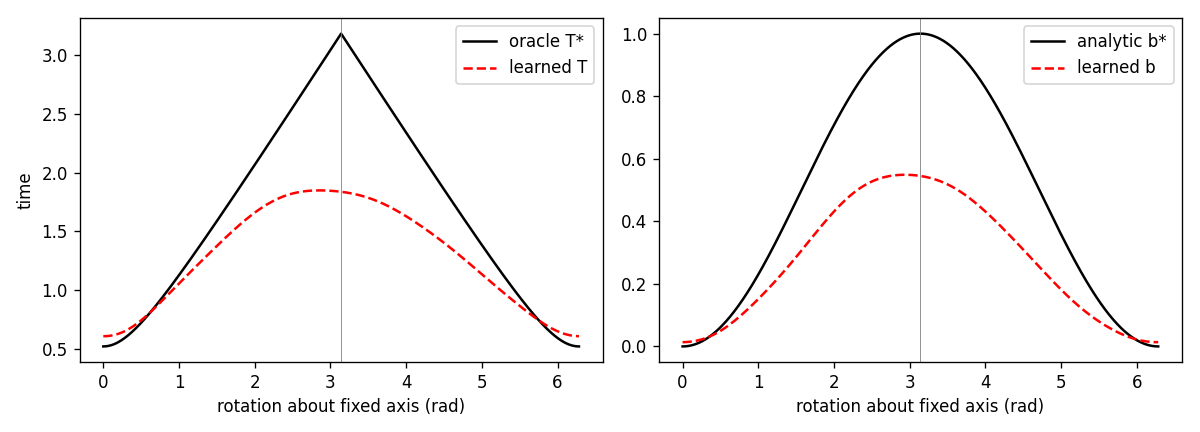
\includegraphics[width=\linewidth]{figures/slice_early_physics.png}
\caption{early physics run (3k steps): $b$ peaks at $\approx0.55$}\end{subfigure}\hfill
\begin{subfigure}{0.49\linewidth}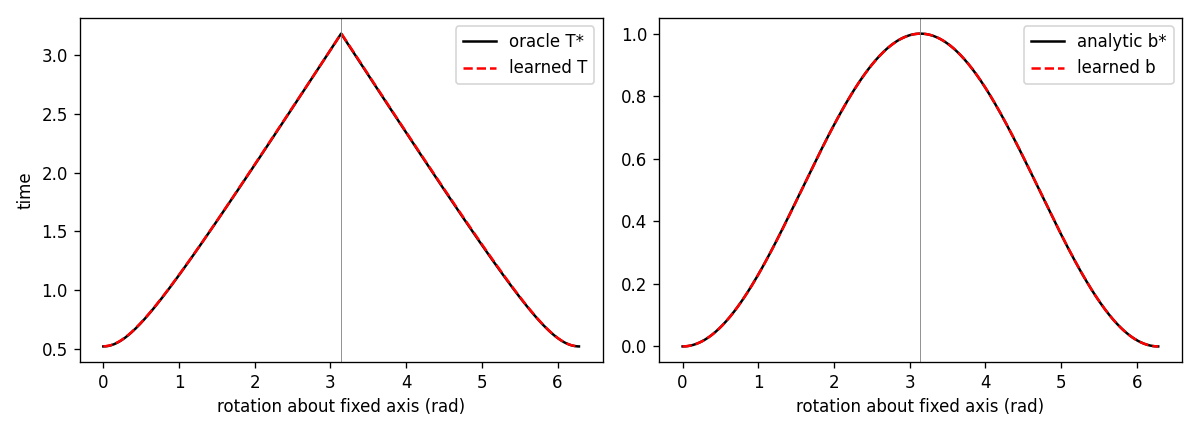
\includegraphics[width=\linewidth]{figures/slice_final_graph_gram.png}
\caption{final \code{graph\_gram}: $b$ reaches 1, corner reproduced}\end{subfigure}
\caption{Travel time (left of each panel) and rotation latent (right) along a slice that rotates the
goal about a fixed axis through the cut locus at $\pi$; black: oracle, red dashed: learned.}
\label{fig:slices}
\end{figure}

\subsection{The correct solution is a stable minimum: warm-start test}

A stage-B checkpoint ($0.11\pct$ / $0.33\pct$) used to initialise physics training stayed in the
correct basin: $1.8\pct$ / $5.1\pct$ at learning rate $10^{-3}$ with anchors, and $0.7\pct$ /
$1.9\pct$ at $10^{-4}$ even \emph{without} anchors (warm-start runs are labelled separately and are
not results). Hence training from scratch failed by reaching a wrong basin, not because the loss is
biased, and gradient noise at $10^{-3}$ costs about two points.

\subsection{Curriculum, cosine decay and input skip}

Restricting the training pairs to relative angles below $\theta_{\max}(k)$ lets the siamese
embedding, which is shared by all pairs, learn the right per-pose structure before the cut locus is
seen. With the input skip and cosine decay, \code{graph\_gram} reached $0.14\pct$ / $0.41\pct$ while
still trained only on pairs up to $160^\circ$, i.e.\ it extrapolated almost exactly to the whole of
$\SO$. Without the skip the same curriculum reached only 17\pct\ at 4k steps; without the curriculum
the skip runs stayed at 4--6\pct; the metric head did not benefit (16\pct).

\subsection{Re-entry of the cut locus and the band sweep}

When the last near-$\pi$ pairs enter $L_E$, $\phi'(b)\to\infty$ makes $(\|c\|^2-1)^2$ spike on a few
samples. \code{graph\_sqdist} did not recover; \code{graph\_gram} dropped to $1.7\pct$ / $4.8\pct$ and
recovered under the decaying learning rate to $0.10\pct$ / $0.32\pct$. A cut-locus band of $10^{-3}$
softens the transient; $10^{-2}$ removes too much supervision ($0.38\pct$ / $0.69\pct$).

\subsection{A degeneracy of physics-only training}

Without anchors, rotations were learned well (pure rotations $0.9\pct$ / $2.7\pct$) but translations
were not ($9.7\pct$ / $66\pct$), with $T/\|\Delta t\|$ down to $0.35$ even for tiny displacements.

\begin{proposition}[Projection-metric degeneracy]\label{prop:degenerate}
Suppose near the diagonal $T(x,x\exp(\widehat{S\delta}))=\sqrt{\delta^\top M\delta}+o(\|\delta\|)$ with
$M\succeq0$. The endpoint Eikonal equation holds for all small $\delta$ if and only if $M^2=M$, i.e.\
$M$ is any orthogonal projection, not only $M=I$.
\end{proposition}
\begin{proof}
To first order $c_x=-M\delta/\sqrt{\delta^\top M\delta}$, so
$\|c_x\|^2=\delta^\top M^2\delta/\delta^\top M\delta$. This equals one for all $\delta$ iff the
symmetric matrix $M^2-M$ vanishes.
\end{proof}

Globally, in a flat analogue $T=\|P(x-y)\|$ with a projection $P$ has $\|\nabla_xT\|=1$ wherever it
is differentiable and spurious zeros on $x+\ker P$. The Bellman minimum selects the steepest action
and never charges a zero-cost direction, so it only lifts the spurious zero set itself, by about $h$
per target update. Declared anchors remove the degeneracy; without labels it is the dominant failure.
A non-detached $e^{-T/2}$ residual weight did not help here.

%=====================================================================
\section{Results: obstacle-free \texorpdfstring{$\SE$}{SE(3)} (stages A--D)}
\label{sec:results}

Tables~\ref{tab:main}--\ref{tab:ablation} report the held-out test set (seed 2002) as mean $\pm$
standard deviation over training seeds 0, 1, 2. Rows marked with one seed are single runs.

\begin{table}[t]\centering\scriptsize\setlength{\tabcolsep}{4pt}
\caption{Field accuracy. Relative errors in \%; ``mix'' is the training mixture (includes small
relative poses and near half-turns); exact-$\pi$ is the mean absolute error on exact half-turns
($T^*\approx3.4$); Eikonal residual is the median $|\|c_x\|^2-1|$ on regular pairs.}
\label{tab:main}
\resizebox{\linewidth}{!}{%
\begin{tabular}{lccccccc}
\toprule
model & seeds & median & 95th pct. & mix 95th & $179$--$180^\circ$ median & exact-$\pi$ abs. & Eikonal res.\\
\midrule
\tabin{tables/main_field.tex}
\bottomrule
\end{tabular}}
\end{table}

\begin{table}[t]\centering\scriptsize\setlength{\tabcolsep}{4pt}
\caption{Planning on 1000 test pairs (identical planners for every field) and metric properties.
Cost ratio = path time / $T^*$. Goal values $T(x,x)$ are exactly 0 for the graph heads, $0.003$ for
the metric heads (their smoothing offset) and $0.057$ for the scalar network; among $10^4$ random
triples no model violates the triangle inequality by more than $10^{-4}$ except the NTFields-loss
metric head ($0.003\pct$ of triples).}
\label{tab:plan}
\resizebox{\linewidth}{!}{%
\begin{tabular}{lccccccc}
\toprule
& & \multicolumn{3}{c}{gradient rollout} & \multicolumn{2}{c}{sampling rollout}\\
\cmidrule(lr){3-5}\cmidrule(lr){6-7}
model & seeds & success \% & cost median & cost 95th & success \% & cost median\\
\midrule
\tabin{tables/main_plan.tex}
\bottomrule
\end{tabular}}
\end{table}

\begin{figure}[t]\centering
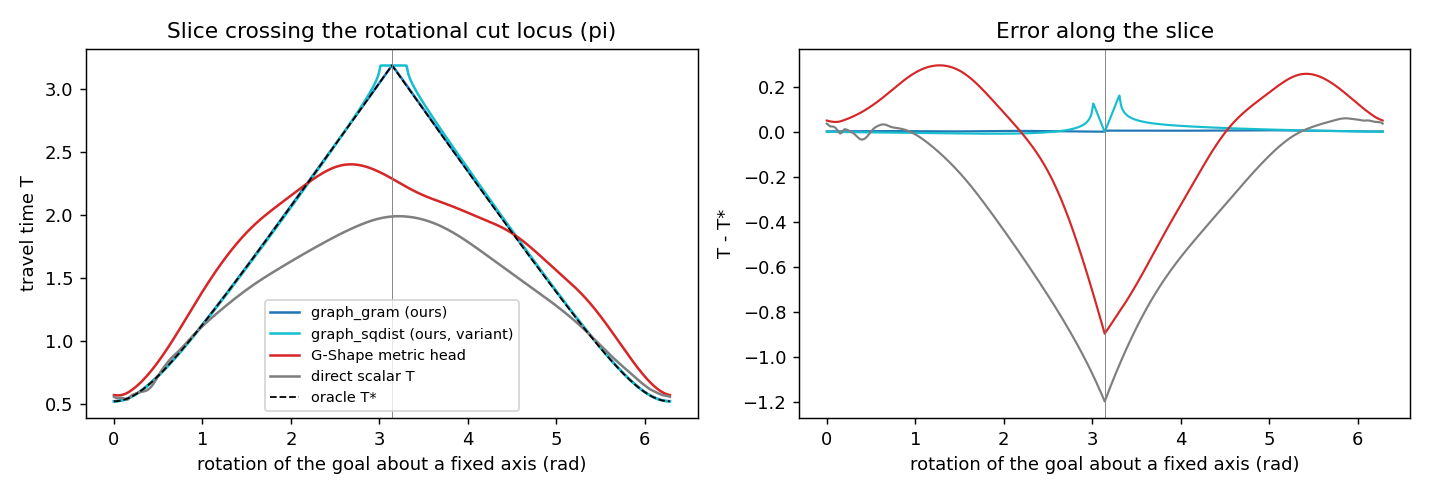
\includegraphics[width=\linewidth]{figures/cut_locus_slice_comparison.png}
\caption{Seed-0 fields along the cut-locus slice of Figure~\ref{fig:slices}. Only the graph heads
form the corner at $\pi$; the metric head and the scalar network are $0.9$ and $1.2$ too low there.
\code{graph\_sqdist} shows a short flat top caused by its saturating adapter.}
\label{fig:slicecmp}
\end{figure}

\begin{figure}[t]\centering
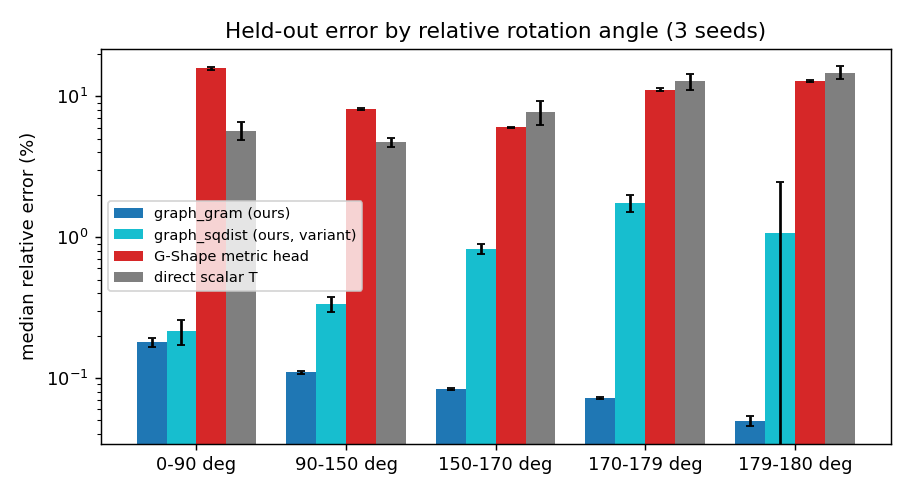
\includegraphics[width=0.78\linewidth]{figures/error_by_angle.png}
\caption{Median relative error by relative rotation angle (log scale, 3 seeds).}
\label{fig:angle}
\end{figure}

\begin{table}[t]\centering\small
\caption{Median relative error (\%) by relative rotation angle (Figure~\ref{fig:angle}).}
\label{tab:angle}
\resizebox{\linewidth}{!}{%
\begin{tabular}{lccccc}
\toprule
model & $0$--$90^\circ$ & $90$--$150^\circ$ & $150$--$170^\circ$ & $170$--$179^\circ$ & $179$--$180^\circ$\\
\midrule
\tabin{tables/angle.tex}
\bottomrule
\end{tabular}}
\end{table}

\begin{table}[t]\centering\scriptsize\setlength{\tabcolsep}{4pt}
\caption{Ablations of the \code{graph\_gram} recipe, the stage-B supervised reference and the stage-E
hybrid head on the obstacle-free benchmark. Columns as in Tables~\ref{tab:main} and \ref{tab:plan}.}
\label{tab:ablation}
\resizebox{\linewidth}{!}{%
\begin{tabular}{lccccccc}
\toprule
variant & seeds & median & 95th pct. & mix 95th & $179$--$180^\circ$ median & exact-$\pi$ abs. & Eikonal res.\\
\midrule
\tabin{tables/ablation_field.tex}
\bottomrule
\end{tabular}}\\[6pt]
\resizebox{\linewidth}{!}{%
\begin{tabular}{lccccccc}
\toprule
variant & seeds & grad.\ succ.\ \% & cost med. & cost 95th & samp.\ succ.\ \% & cost med.\\
\midrule
\tabin{tables/ablation_plan.tex}
\bottomrule
\end{tabular}}
\end{table}

\paragraph{Findings (empirical, this benchmark).}
\begin{itemize}
\item The smooth-graph field is about $90\times$ more accurate than the G-Shape metric head under
identical conditions and plans optimally (cost ratio 1.0000 vs.\ 1.12). It meets the specification's
provisional gates on every seed.
\item The mechanism is confirmed at the cut locus. The error of \code{graph\_gram}
\emph{decreases} toward $180^\circ$, the decoded time has the corner (slice error
$\le\slicepi$ near $\pi$), and the latents match the analytic ones without latent supervision
(median $|a-a^*|=\latentA$, $|b-b^*|=\latentB$). This identifiability was observed, not
guaranteed.
\item Exact goal values matter for planning. The direct scalar network cannot be planned on with
the gradient rollout ($1.4\pct$ success): without an exact zero its minimum is offset from the goal.
\item Required ingredients: the curriculum (without: $4.0\pct$), the input skip (without:
$11.8\pct$) and the anchors (without: $2.4\pct$ / $19\pct$, Proposition~\ref{prop:degenerate}).
\item The Bellman term, as configured, slightly \emph{hurts} final accuracy ($0.072\pct$ without vs.\
$0.105\pct$ with). It is kept in the main row because the specification's objective includes it.
Finite candidate sets bias $\mathcal BT$ upward, and the lagged EMA target slows convergence.
\end{itemize}

%=====================================================================
\section{Stage E: obstacles}
\label{sec:stagee}

The specification allows this only after stages A--D and warns that the two-output decoder then no
longer implies smooth targets or physical meanings for $a$ and $b$. Everything in this section is
empirical.

\subsection{Setup}

\paragraph{Data and speed model.}\sloppy The preprocessed 3D-shape datasets of the repository
(in \code{datasets/3dshape/}, $8\times10^5$ pose pairs each, rotations stored as
rotation vectors divided by $2\pi$) provide clearance speeds $s\in(0,1]$ per endpoint. We use the
declared position-dependent ellipsoidal model
\begin{equation}
\frac{\|v\|^2}{(S(x)s_t)^2}+\frac{\|\omega\|^2}{(S(x)s_r)^2}\le1,\qquad s_t=1,\ s_r=2\pi,\qquad
S=w(s)=s^2(2-s)^2,
\end{equation}
i.e.\ rotations are measured in turns as in the baseline, and $w$ is the baseline's speed warp
applied to the combined (isotropic) speed. The endpoint Eikonal equations become
$\|S(x)\,c_x\|=\|S(y)\,c_y\|=1$ with $c$ computed by \eqref{eq:proj}.\fussy

\paragraph{Loss.} No oracle and no anchors exist. Following NTFields we use the residual
$r_x=(\|S(x)c_x\|^{1/2}-1)^2$ and the weight $e^{-T/2}$ \emph{without} detaching $T$:
\begin{equation}
L=\mathbb E\bigl[(r_x+r_y)\,e^{-T_\theta/2}\bigr],\qquad
\nabla_\theta L=\mathbb E\bigl[e^{-T_\theta/2}\nabla_\theta(r_x+r_y)\bigr]
-\tfrac12\,\mathbb E\bigl[(r_x+r_y)\,e^{-T_\theta/2}\,\nabla_\theta T_\theta\bigr].
\end{equation}
The second term pushes $T$ up wherever the residual is large, an implicit anti-collapse force
(Proposition~\ref{prop:degenerate}). There is no Bellman term (the baseline runs with TD off). AdamW
(weight decay 0.5, learning rate $5\times10^{-4}$), batch 2000, 20\,000 updates, Fourier
$\sigma_t=0.5$ for translation and $\sigma_r=0.1$ for rotation columns
(\code{configs/graph\_method/stageE\_common.json}). All heads use exactly this pipeline.

\paragraph{Evaluation.} The unmodified Shape-NTFields evaluator (\code{evaluate\_training\_3d\_batched.py}:
MPPI in $(t,\text{rotvec}/2\pi)$ coordinates, collision checks against the environment mesh, 1000
RRT-verified start/goal pairs) queries our fields through a small adapter
(\code{shape\_adapter.py}). It reports four planner variants (forward, reverse, either-of-the-two,
alternate) and failure counts (collision, non-convergence; they can overlap).

\subsection{Getting the pipeline to work}

Table~\ref{tab:explore} lists the exploration on the first 200 test cases (one seed each; standard
error about 3 points). The first fields failed completely (0--1\pct; every episode failed to converge).
Two diagnostics located the problem. (i) Since $S\le1$, the obstacle-free time is a lower bound,
$T\ge T_{\mathrm{free}}$; the working baseline field has $T/T_{\mathrm{free}}\approx3.0$ (5th--95th
percentile 2.4--4.1) on test pairs, ours had 0.55--1.3. (ii) Binned by clearance speed, the
baseline's $S\|\nabla T\|$ has medians $0.13,0.63,1.08,1.44$ for $S\in[0,0.01),[0.01,0.1),[0.1,0.5),
[0.5,1)$; ours had $0.025,0.24,1.09,2.0$: a nearly speed-independent gradient that ignores the
clearance structure. With $c=S\nabla T$ the spec residual's push on $\|\nabla T\|$ scales like $S^2$
($\approx3\times10^{-6}$ in the clearance band). The non-detached weight (0--1\pct\ $\to22\pct$), the
input skip ($6\pct\to22\pct$) and above all the rotation frequency (with $G(x)$ containing
$\vecop R$, $\sigma_r=0.3$ gives about $3\times$ the phase per radian of the baseline's rotation-vector
input; $\sigma_r=0.1$: $22\pct\to67$--$69\pct$; then $\sigma_t=0.5$: $77$--$79\pct$) fixed it.
Anisotropic speeds hurt (11\pct); a hinge penalty for $T\ge T_{\mathrm{free}}$ did not help.

\begin{table}[t]\centering\scriptsize
\caption{Stage E exploration on Tshape3d\_env1, first 200 test cases, forward MPPI. $\sigma$ column:
Fourier $\sigma_t/\sigma_r$ (single value: coordinate inputs). The last block calibrates against a
replica of the baseline pipeline and the baseline checkpoint itself.}
\label{tab:explore}
\resizebox{\linewidth}{!}{%
\begin{tabular}{lllccc}
\toprule
head & setting & $\sigma$ & success \% & collision & no-conv.\\
\midrule
\tabin{tables/stageE_explore.tex}
\bottomrule
\end{tabular}}
\end{table}

\subsection{The translation-type latent: Euclidean vs.\ metric}

With the matched pipeline the metric head led \code{graph\_gram} by about five points. For
\code{graph\_gram}, $T^2-\phi(b)/s_r^2=\|A(e_x-e_y)\|^2$ is a squared Euclidean embedding distance,
while the rotation term is bounded:
\begin{equation}
0\le\frac{\phi(b)}{s_r^2}\le\frac{\pi^2}{(2\pi)^2}=\frac14 .
\end{equation}
All extra time caused by obstacles must therefore be expressed as a Euclidean distance between
embeddings. A finite metric is isometrically $\ell_2$-embeddable only if
$-\tfrac12JD^{(2)}J\succeq0$ (Schoenberg), which geodesic distances in non-convex domains can
violate, whereas every finite metric embeds isometrically into $\ell_\infty$ (Fr\'echet), the
structure of \eqref{eq:metric}. The hybrid \code{graph\_metric} keeps the graph latents and decoder but
takes $a$ from the metric distance. Widening the Euclidean latent instead ($k_a=128$) did not help.
The hybrid is not a universal head: on the obstacle-free benchmark it reaches only $8.7\pct$ median
error (Table~\ref{tab:ablation}). Because the $b$ term is bounded by $1/4$, among obstacles the hybrid
is essentially the metric head plus a graph-style rotation term, so its parity shows that the graph
structure costs nothing there, not that it helps.

\subsection{Results}

\begin{table}[t]\centering\scriptsize\setlength{\tabcolsep}{4pt}
\caption{Stage E, all 1000 test cases per environment, success (\%) per MPPI variant and failure
counts of the forward planner. $^\dagger$Native NTFields pipeline, checkpoints of seeds 1 and 2
(Lie-Shape-NTFields, epoch 4000) with the same evaluator and test set; its research notes report
$81.9\pm0.5\pct$ over five seeds on this environment.}
\label{tab:stagee}
\resizebox{\linewidth}{!}{%
\begin{tabular}{lccccccc}
\toprule
model & seeds & forward & reverse & either & alternate & collision & no-conv.\\
\midrule
\multicolumn{8}{l}{\emph{Tshape3d\_env1}}\\
\tabin{tables/stageE_T.tex}
\midrule
\multicolumn{8}{l}{\emph{Lshape3d\_env3}}\\
\tabin{tables/stageE_L.tex}
\midrule
\multicolumn{8}{l}{\emph{Ashape3d\_env4}}\\
\tabin{tables/stageE_A.tex}
\bottomrule
\end{tabular}}
\end{table}

Table~\ref{tab:stagee} gives the final comparison. Inside one pipeline \code{graph\_metric} is on par
with the metric head: $79.2$ vs.\ $80.0\pct$ forward on the T-shape (equal or better on the three other
planner variants), $82.9$ vs.\ $81.4\pct$ on the L-shape and $81.5$ vs.\ $81.5\pct$ on the A-shape
(mean $81.2$ vs.\ $81.0\pct$). \code{graph\_gram} is 5--11 points behind. The metric head inside our
pipeline matches the native baseline within about one point on the T-shape, so the pipeline is
validated. The native pipeline is still ahead there, by 1.2 (metric head), 2.0 (\code{graph\_metric}) and
6.1 (\code{graph\_gram}) points against its two re-scored checkpoints (more against its five-seed mean),
and it fails differently (about 118 collisions vs.\ about 20 for ours). Research notes report 88--92\pct\ (L) and 86--89\pct\
(A) for it. The remaining gap was not attributable to the NTFields accept/reject rollback (it never
triggered), gradient clipping, the regular-sample mask or the Fourier sampling scheme
(Table~\ref{tab:explore}); it remains unexplained. Lshape3d\_env3 and Ashape3d\_env4 were scored with
the Lie-Shape-NTFields copy of the same evaluator (identical code path, byte-identical test sets),
because the Shape-NTFields checkout lacks those meshes.

%=====================================================================
\section{Discussion}

\paragraph{Established vs.\ empirical.}
Proven or verified to numerical precision: the identities of Section~\ref{sec:formulation}, the
tangent projection, the Eikonal equations of the oracle, Proposition~\ref{prop:gram} and
Proposition~\ref{prop:degenerate}. Empirical, on this benchmark only: every learned result. Not
established: convergence of sampled PDE training to the viscosity solution in general,
identifiability of $(a,b)$, the triangle inequality (measured, not guaranteed), any claim of
superiority among obstacles.

\paragraph{Deviations from the specification} (all tuned on validation data only).
\begin{itemize}
\item Batch 1024 instead of 256 (same wall-clock cost; training is kernel-launch bound) and 12k
instead of 20k updates.
\item Bellman step $h=0.2\,\taur$.
\item The relative-angle curriculum and the input skip.
\item Training is in float32; geometry verification is in float64.
\item Stage E uses the NTFields residual form and weighting, isotropic speeds, no Bellman term and no
anchors.
\end{itemize}

\paragraph{Limitations.} The obstacle-free benchmark has an analytic solution; success validates the
representation and its optimisation, not a need for learning. Physics-only training without labels
does not reach the accuracy of the anchored version because of the degeneracy of
Proposition~\ref{prop:degenerate}. The curriculum uses the relative rotation angle of the pair, which
is input geometry but specific to the rotational structure. Stage E has one environment with three
seeds and two with two seeds, and an unexplained gap to the native pipeline.

\paragraph{Future work.} (i) One head for both settings, e.g.\ $a=\|A(e_x-e_y)\|^2+m^2$, letting the
network use whichever channel fits; (ii) constraints that remove the projection-metric degeneracy so
physics-only training works without anchors; (iii) Bellman targets without upward bias (more or
optimised candidates, multi-step rollouts); (iv) closing the gap to the native NTFields pipeline;
(v) more environments and seeds.

%=====================================================================
\section{Reproducibility}

All code runs inside the \code{pytorchserver:latest} image (PyTorch 2.2.2, CUDA 12.1) from the
repository root.
{\footnotesize
\begin{verbatim}
python -m unittest tests.test_graph_method                         # stage A
python -m models.graph_method.evaluate --analytic --out results/graph_method/analytic
python train/train_graph.py --config configs/graph_method/graph_gram.json --seed 0 \
    --out_root ./Experiments/graph_method_final
python -m models.graph_method.evaluate \
    --ckpt Experiments/graph_method_final/graph_gram_s0/best.pt \
    --out results/graph_method_final/graph_gram_s0
python train/train_graph.py --config configs/graph_method/stageE_common.json --seed 0 \
    --name stageE_graph_metric_s0 --out_root ./Experiments/graph_method_stageE \
    --set fourier_sigma_t=0.5 fourier_sigma_r=0.1 arch=graph_metric skip_input=True
python models/graph_method/scripts/run_shape_eval.py /shape /workspace \
    --dataPath testing_data/3dshape/Tshape3d_env1 --no-viser --cases 0 \
    --checkpoint /workspace/Experiments/graph_method_stageE/stageE_graph_metric_s0/latest.pt \
    --out /workspace/results/graph_method_stageE/stageE_graph_metric_s0_c1000
python3 models/graph_method/report/make_tables.py                  # tables of this report
\end{verbatim}
}
{\sloppy\noindent The package layout follows the specification's contract: \code{geometry/} (se3, tangents),
\code{fields/} (oracle, decoder), \code{interface.py}, \code{model\_network\_graph.py} (encoder and
heads), \code{losses/} (eikonal, bellman), \code{data/poses.py}, \code{planning/rollout.py},
\code{model\_function\_graph.py} and \code{model\_train\_graph.py} (losses, training, checkpoints
with optimiser, EMA, sampler and RNG states, scales, exclusions and code revision),
\code{evaluate.py}, \code{model\_function\_shape.py} and \code{shape\_adapter.py} (stage E),
\code{tests/test\_graph\_method.py} and \code{configs/graph\_method/}. All tables in this report are
generated from the saved evaluation files by \code{report/make\_tables.py}.\par}

\appendix
\section{Hyperparameters}

\begin{center}\small
\begin{tabular}{lll}
\toprule
& obstacle-free (\code{graph\_gram.json}) & stage E (\code{stageE\_common.json})\\
\midrule
speed scales $s_t,s_r$ & $1,1$ & $1,2\pi$ (position-dependent $S(x)$)\\
encoder & 256 wide, 2 gated blocks, skip & same\\
Fourier $\sigma$ & $0.03$ (all columns), clipped & $\sigma_t=0.5$, $\sigma_r=0.1$, resampled\\
heads & \code{graph\_gram}: $k_a=16$, $4\times4$ Gram & \code{graph\_gram}, \code{graph\_metric}, metric\\
objective & $L_E+L_B+10L_{\mathrm{goal}}+L_T$ & $\mathbb E[(r_x+r_y)e^{-T/2}]$\\
Eikonal residual & $(\|c\|^2-1)^2$ & $(\|Sc\|^{1/2}-1)^2$\\
anchors & 1024 (seed 777) & none\\
Bellman & $h=0.2$, 32 candidates, EMA 0.995 & none\\
bands & $T^*/\taur\ge10^{-3}$, $1-b^*\ge10^{-4}$ & $T_{\mathrm{free}}\ge10^{-3}$, $1-b_{\mathrm{free}}\ge10^{-3}$\\
curriculum & $60^\circ\to180^\circ$ over 7k updates & none\\
optimiser & Adam, cosine $10^{-3}\to5\times10^{-5}$ & AdamW, wd 0.5, $5\times10^{-4}$\\
batch / updates & 1024 / 12\,000 & 2000 / 20\,000\\
gradient clipping & 1.0 & 1.0\\
selection & best validation score & last checkpoint\\
\bottomrule
\end{tabular}
\end{center}

\end{document}
